\documentclass[spanish]{llncs}   % llncs.cls esta en la ruta predefinida de TEX Live
\usepackage[colorlinks,citecolor=black,urlcolor=black,linkcolor=black,bookmarks=false,hypertexnames=true]{hyperref}
\usepackage{listingsutf8}
\usepackage{graphicx}


\begin{document}
\title{Práctica 9 - Tripletas RDF}

\author{Hugo Pérez Fernández.  \email{UO250708@uniovi.es}
\institute{Sistemas de Información para la Web. Grado de Ingeniería Informática. EII. 
universidad de Oviedo. Campus de los Catalanes. Oviedo.}}
\maketitle              

\section{Introducción}


\section{Obtención manual de información estructurada}

Primero obtendremos toda la información estructurada de los textos indicados en el Anexo.\ref{Textos}, usando para ello la web \href{https://schema.org}{Schema.org}:

\paragraph{Texto 1:}

En el caso de este texto se esta mecionando a una persona (\textit{schema:Person}), cuyo nombre es Miles Davis, ademas esta persona tiene como nacionalidad \textit{schema:Nacionality}
Americano (Estadounidense), y su profesión (\textit{schema:Ocupation}) es músico concretamente de Jazz.

\paragraph{Texto 2:}

En en este caso la información se puede estructurar de la siguiente forma:

\begin{itemize}
    \item Hay y una persona (\textit{schema:Person}) que se llama Barack Obama cuya ocupación (\textit{schema:Ocupation}) es presidente.
    \item Hay una organizacion (\textit{schema:Organization}) que se llama Unión Europea.
    \item Hay una ciudad (\textit{schema:City}) que se llama Washington.
    \item Hay una tipo de cambio de moneda (\textit{schema:ExchangeRateSpecification}) que se llama Euro y tiene un valor de 1.3.
    \item Hay una reunion (\textit{schema:BusinessEvent}) entre Barack Obama y la Unión Europea
    sobre el el valor del tipo de cambio del Euro.
\end{itemize}

\paragraph{Texto 3:}

En este último se  puede estructura la información del siguiente modo:

\begin{itemize}
    \item Hay una organización (\textit{schema:Organization}) que se llama The New York Times.
    \item Hay una persona (\textit{schema:Person}) que se llama Jhon McCarthy.
    \item Jhon McCarthy está muerto.
    \item El New York Times informa (\textit{schema:Report}) que Jhon McCarthy esta muerto.
    \item LISP es un lenguaje de programación.
    \item John McCarthy inventó LISP.
\end{itemize}

Con los datos obtenidos anteriormente se, usando la notacion Turtle, la información estructurada queda de la siguiente manera:

\lstset{
    frame=tb, % draw a frame at the top and bottom of the code block
    tabsize=2, % tab space width
    showstringspaces=false, % don't mark spaces in strings
    numbers=left, % display line numbers on the left
    commentstyle=\color{green}, % comment color
    keywordstyle=\color{black}, % keyword color
    stringstyle=\color{blue}, % string color    
    inputencoding=utf8/latin1
}
\lstinputlisting[language=HTML, breaklines, caption={Archivo Turtle con la información estructurada de los textos.}]{resources/texts.ttl}

Ahora verificaremos la estructura de la sistaxis RDF de del archivo anterior mediante la herramienta \href{http://rdfshape.weso.es/dataInfo}{RDFShape}:

\begin{figure}[h]
    \centering
    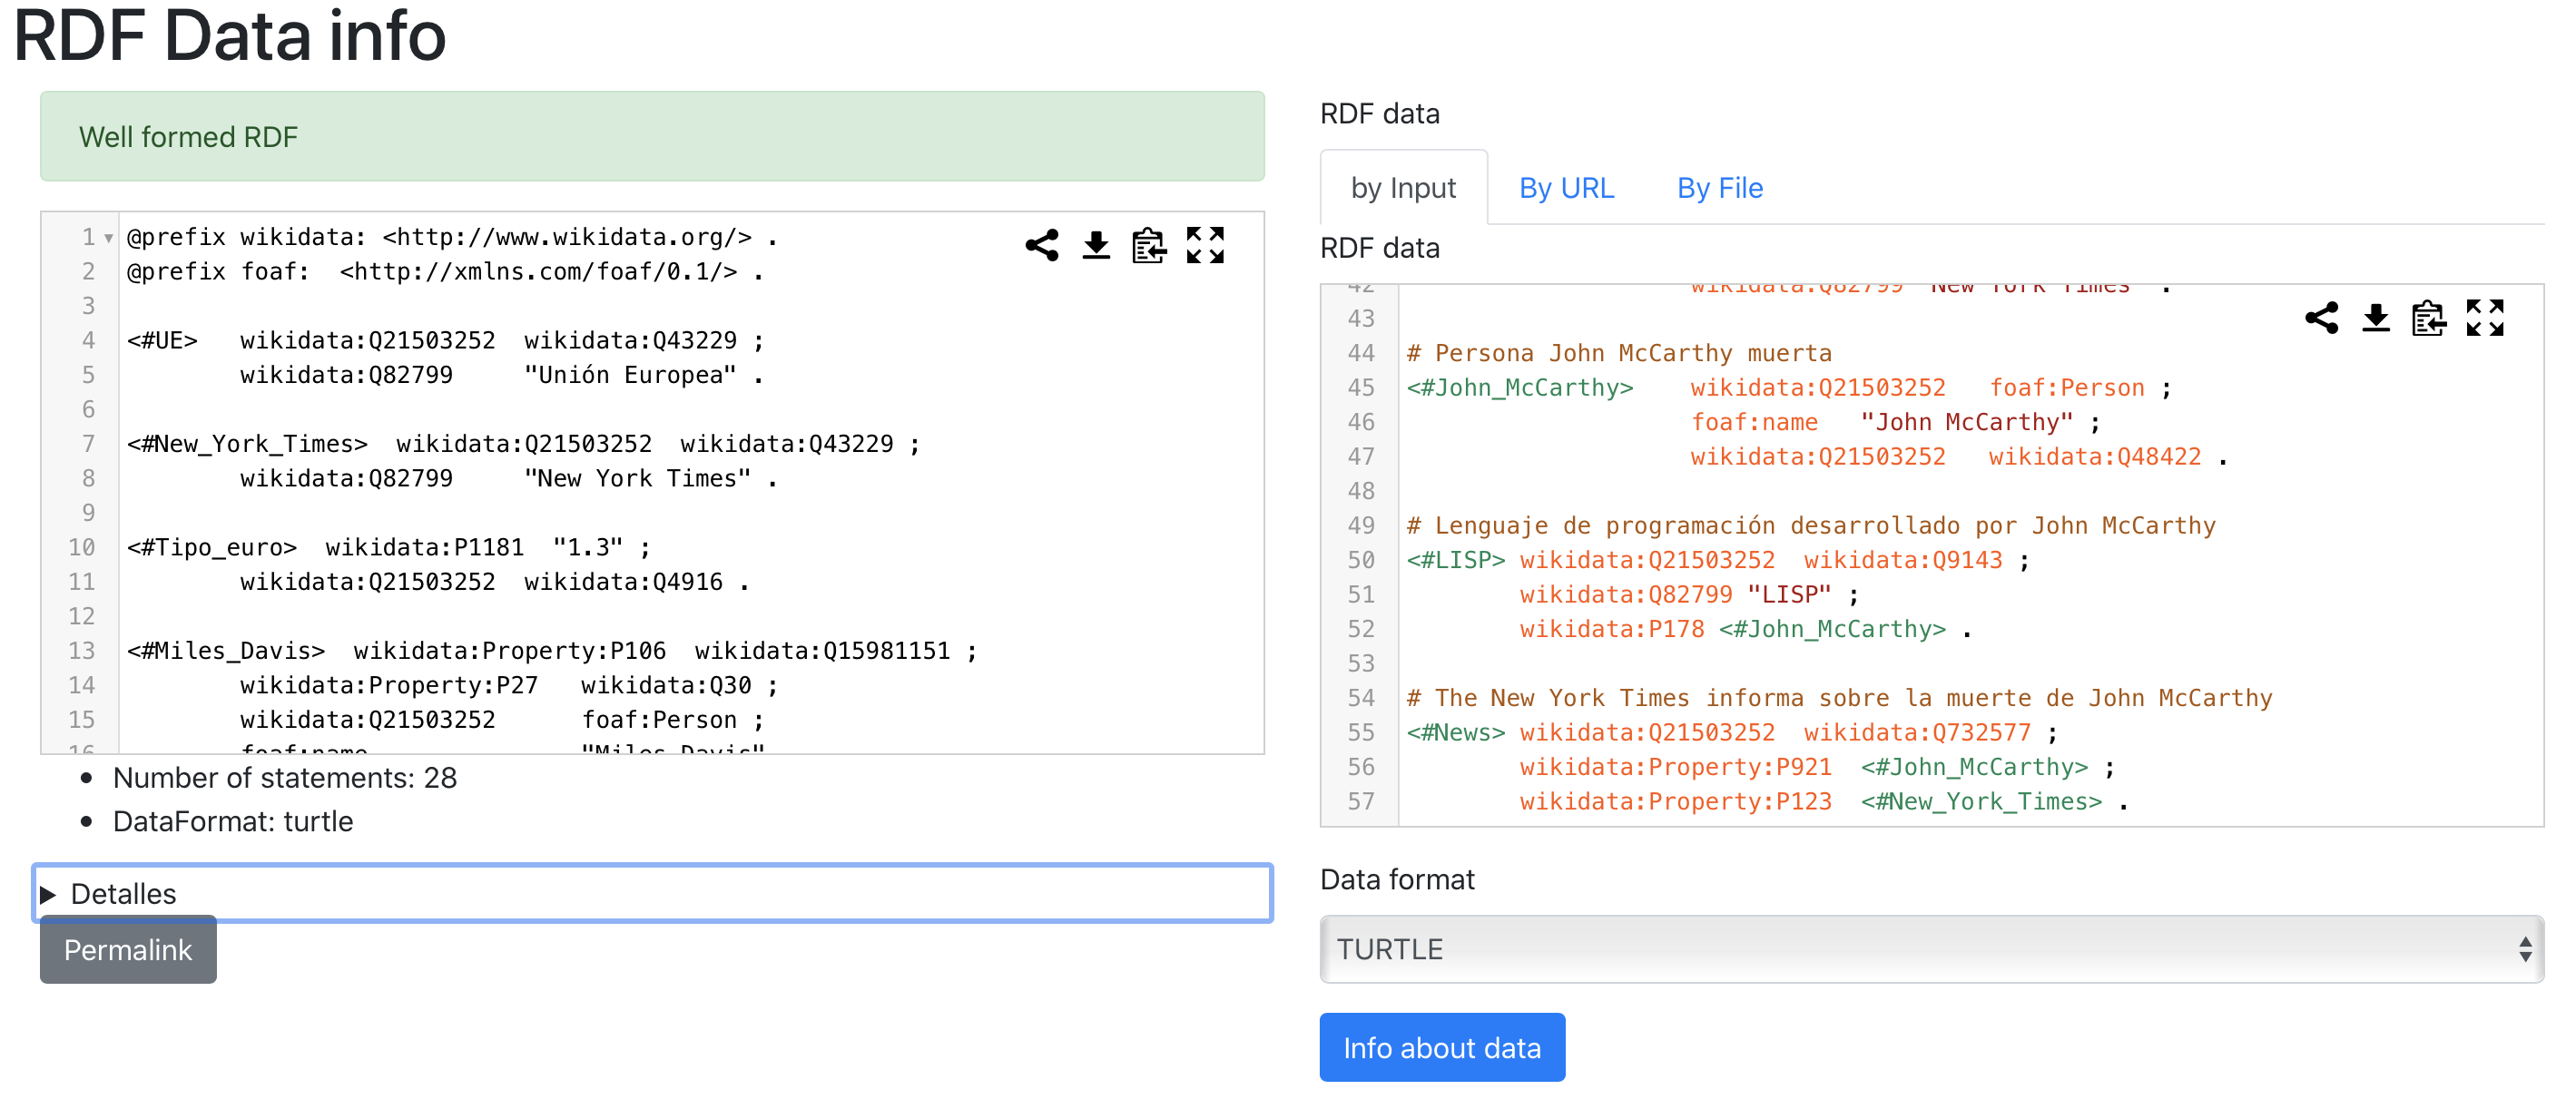
\includegraphics[width=\textwidth]{resources/RDFValidation.png}
    \caption{Resultado de la validación del ttl con RDFShape.}
    \label{Fig.1}
\end{figure}

Una vez verificado podemos traducir el formato turtle a JSONLD, usando para ello la herramienta \href{https://rdf-translator.appspot.com}{RDF-Translator}, de forma que quedaria de la siguiente manera:

\lstset{
    frame=tb, % draw a frame at the top and bottom of the code block
    tabsize=2, % tab space width
    showstringspaces=false, % don't mark spaces in strings
    numbers=left, % display line numbers on the left
    commentstyle=\color{green}, % comment color
    keywordstyle=\color{red}, % keyword color
    stringstyle=\color{black}, % string color    
    inputencoding=utf8/latin1
}
\lstinputlisting[language=HTML,breaklines,caption={Archivo Resultado de la traduccion de turtle a JSONLD.}, captionpos=b]{resources/jsonld.json}


\section{Obtención automática de información estructurada}

\subsection{Obtención de RDF's.}

Obtendremos los documentos RDF para cada texto, par ello usaremos las siguientes herramientas: 
\href{https://www.refinitiv.com/en/products/intelligent-tagging-text-analytics}{Open Calais}, 
\href{https://www.dbpedia-spotlight.org/demo/}{DBPedia-spotlight} y 
\href{http://wit.istc.cnr.it/stlab-tools/fred/demo/?}{FRED} 
estos se pueden ver correspondientemente en los Anexos: \ref{OpenCalaisRDF}, \ref{DBPediaRDF} y \ref{FREDRDF}.



\section{Anexos}

\subsection{Textos de Prueba}\label{Textos}

\paragraph{Texto 1:}
“Miles Davis was an american jazz musician.”

\paragraph{Texto 2:}
“President Barack Obama and European Union leaders huddled in Washington amid growing fears over the future of the euro, which closed greater than 1.3 dollars.”

\paragraph{Texto 3:}
“The New York Times reported that John McCarthy died. He invented the programming language LISP.”

\subsection{Archivos RDF producidos por herramientas}

\subsubsection{Open Calais}\label{OpenCalaisRDF}
%\lstinputlisting[language=XML, firstline=1, lastline=25, breaklines, caption={Archivo RDF con la información estructurada del texto 1.}]{resources/OpenCalaisText1.rdf}
%\lstinputlisting[language=XML, lastline=50, breaklines, caption={Archivo RDF con la información estructurada del texto 2.}]{resources/OpenCalaisText2.rdf}
%\lstinputlisting[language=XML, lastline=50, breaklines, caption={Archivo RDF con la información estructurada del texto 3.}]{resources/OpenCalaisText3.rdf}

\subsubsection{DBPedia-Spotlight}\label{DBPediaRDF}
\subsubsection{FRED}\label{FREDRDF}
%\lstinputlisting[language=XML, firstline=1, lastline=25, breaklines, caption={Archivo RDF con la información estructurada del texto 1.}]{resources/FredText1.rdf}
%\lstinputlisting[language=XML, lastline=50, breaklines, caption={Archivo RDF con la información estructurada del texto 2.}]{resources/FredText2.rdf}
%\lstinputlisting[language=XML, lastline=50, breaklines, caption={Archivo RDF con la información estructurada del texto 3.}]{resources/FredText3.rdf}

\end{document}